\glsresetall{} 
\chapter{Software Architecture}


\section{Payload Operations Planning Software Architecture}

The \gls{pops} is made up of several distinct components separated into
services.  Each service has its own Docker5 container. Containers are similar
to virtual machines in that they simulate an operating system but, unlike
virtual machines, they do not simulate the underlying hardware. This makes
containers much more lightweight, while also retaining the benefits of having a
standardized environment where dependencies are packaged with their source
code. Containers make deploying and maintaining \gls{pops} much easier since
installation does not require managing dependencies and tweaking environment
variables. In this way, a \gls{pops} user does not need to be as familiar with
the software as a developer to run it. Each service is its own Python web
server. In this way, they may be interacted with via a RESTful API. That being,
HTTP requests can be made to retrieve information or perform calculations. Each
service also provides its own automatically generated documentation that can be
accessed through a web browser. This documentation outlines possible API calls
as well as their input and output data formats.  This allows a user to quickly
see the capabilities of a service without accessing the source code. Currently,
\gls{pops} has 4 main services; they are the: Mission Model, Propagator,
Database, and Access Time Utilities,  Mission Model.

\section{General Service Architecture}

Every service contains the same basic components so it is worth discussing
services generally and then going into specifics in subsequent sections. These
components are: the dockerfile, a main Python script, a models file, service
specific scripts.

To review, a docker container is a virtual environment, which is a simulated
operating system. A container can be created from an image and an image canbe
built from a Dockerfile. As such, the Dockerfile is the fundamental text
document that is used to assemble an image. It specifies: the operating system
that should be used, what files should be included in the container, and what
commands should be run upon container creation. By specifying an operating
system, we can tailor a service to any environment that best suits the service's
needs. They can use windows, the latest version of Ubuntu, or a lightweight
tailored linux distrubution that only contains the tools a service needs. In
this way, one service can be running Ubuntu 20.04 for ease of development, and
another service can be running Windows 10. In this way, \gls{pops} is not
limited by the operating system it is developed in. Files may  be added to a
container simply by pointing to their location in the host's file system upon
image creation. Finally, when a container is first created from an image, a
conatiner will need to install all of the necessary dependencies. In general,
this will either be Ubuntu packages, a version of Python, and Python libraries.
In this way, dependencies can easily be tracked. The last command that is
executed is the command that starts a service's main script.

Theoretically, all of the code for a service could live in the main Python file
but, if this were the case, it would quickly balloon and become unwieldy to work
with so functionality is split into multiple scripts. The main script serves a
number of functions. Its purpose is to handle all of the web-server aspects of
the service. Functions such as: creating the web-server, setting server
parameters, setting up environment variables, and handling API calls. Setting up
the webserver is fairly straightforward since open source libraries are used to
handle all of the low-level functionality and implementation. What is most
important is specifying potential HTTP requests. These requests are how a
service may be interacted with by a user, their browser, or by other services.
The parts that must be specified are the: 

\begin{itemize}
    \item Request type (GET, POST, PUT, etc.), 
    \item Path to the request, 
    \item Response type (JSON, Plain Text, HTML, etc.), 
    \item Input variables if applicable, and the 
    \item Function that is called when a request is received.
\end{itemize}

For GET requests, the input variables are generally straightforward since the
only input variables that can be used must be explicitly stated in the request
itself. But, for POST requests or other requests that contain information in
the body of the request, the format of the input data must be defined or else
the web server will fail the request as being unprocessable. These input
definitions are stored in the models file. Python is a dynamically typed
language so variables do not need to be assigned a type upon creation. To
ensure input data conforms with what is expected by the api, the Python library
\texttt{Pydantic} is used to enforce data types at runtime. These Pydantic
input definitions are contained in the models file. The remainder of the files
in a service are specific to the service itself.

Having multiple Docker containers becomes cumbersome when a user or a developer
wishes to build new images or run new containers from their images. To manage
all of the different services, another tool is used called "Docker Compose".
From a single configuration file, mutliple services may be started, stopped, or
built from their source code. Services may also have their image name,
container name, and port number set through the configuration file. This vastly
simplies configuration for \gls{pops} as a whole. Another benefit of using
Docker Compose is that it also creates a bridget network for the containers
Docker Compose creates. Containers are intended to be standalone units but a
bridge network allows containers to communicate with each other directly.


\section{Propagator Service}

The Propagator service handles ephemeris generation for \gls{pops}.
Ephemerides are a crucial component for every subsequent step along the
planning process so it is essential that they are well formed. Consolidating
ephemeris generation for the entire tool ensures that only one area of the code
needs to be developed and validated.

Currently, the main method of orbital propagation for \gls{pops} is with the
\gls{sgp} model series of algorithms, specifically SGP4/SDP4 referred to as
just ‘SGP4’. SGP4 is an analytical method of approximating orbital state
vectors at corresponding epochs in the \gls{teme} \gls{eci} coordinate frame,
given a NORAD \gls{tle}.  \gls{tle}s are readily provided by the United States
Space Force through Space-Track6 or CelesTrak7. The \gls{teme} coordinate frame
is not particularly useful so part of the Propagator service’s purpose is
transforming the orbit vectors into a coordinate system required by other parts
of \gls{pops}.  Currently, the two possible output reference frames are the
\gls{gcrs}, which is an \gls{eci} reference frame, and the \gls{wgs}, which is
an \gls{ecef} reference frame.  Depending on the application, it is sometimes
useful to use \gls{eci} or \gls{ecef} reference frames, so both are made
available by the service.  Given a \gls{tle}, a time range, a step size, and a
coordinate system, the Propagator service generates an Ephemeris for the
provided time range in a variety of output formats.

There are two scripts that handle all of the functionality for the Propagator
service. The first is the main script which, as discussed previously, takes
requests, organizes the input data, and formats the output data. The actual
propagation and coordinate change logic is stored in the propagation script.
Open source libraries are used to perform the SGP4 and coordinate change
algorithm so the main focus of the script is to ensure the input data conforms
with the expected format.  

\begin{figure}[h]
    \centering
    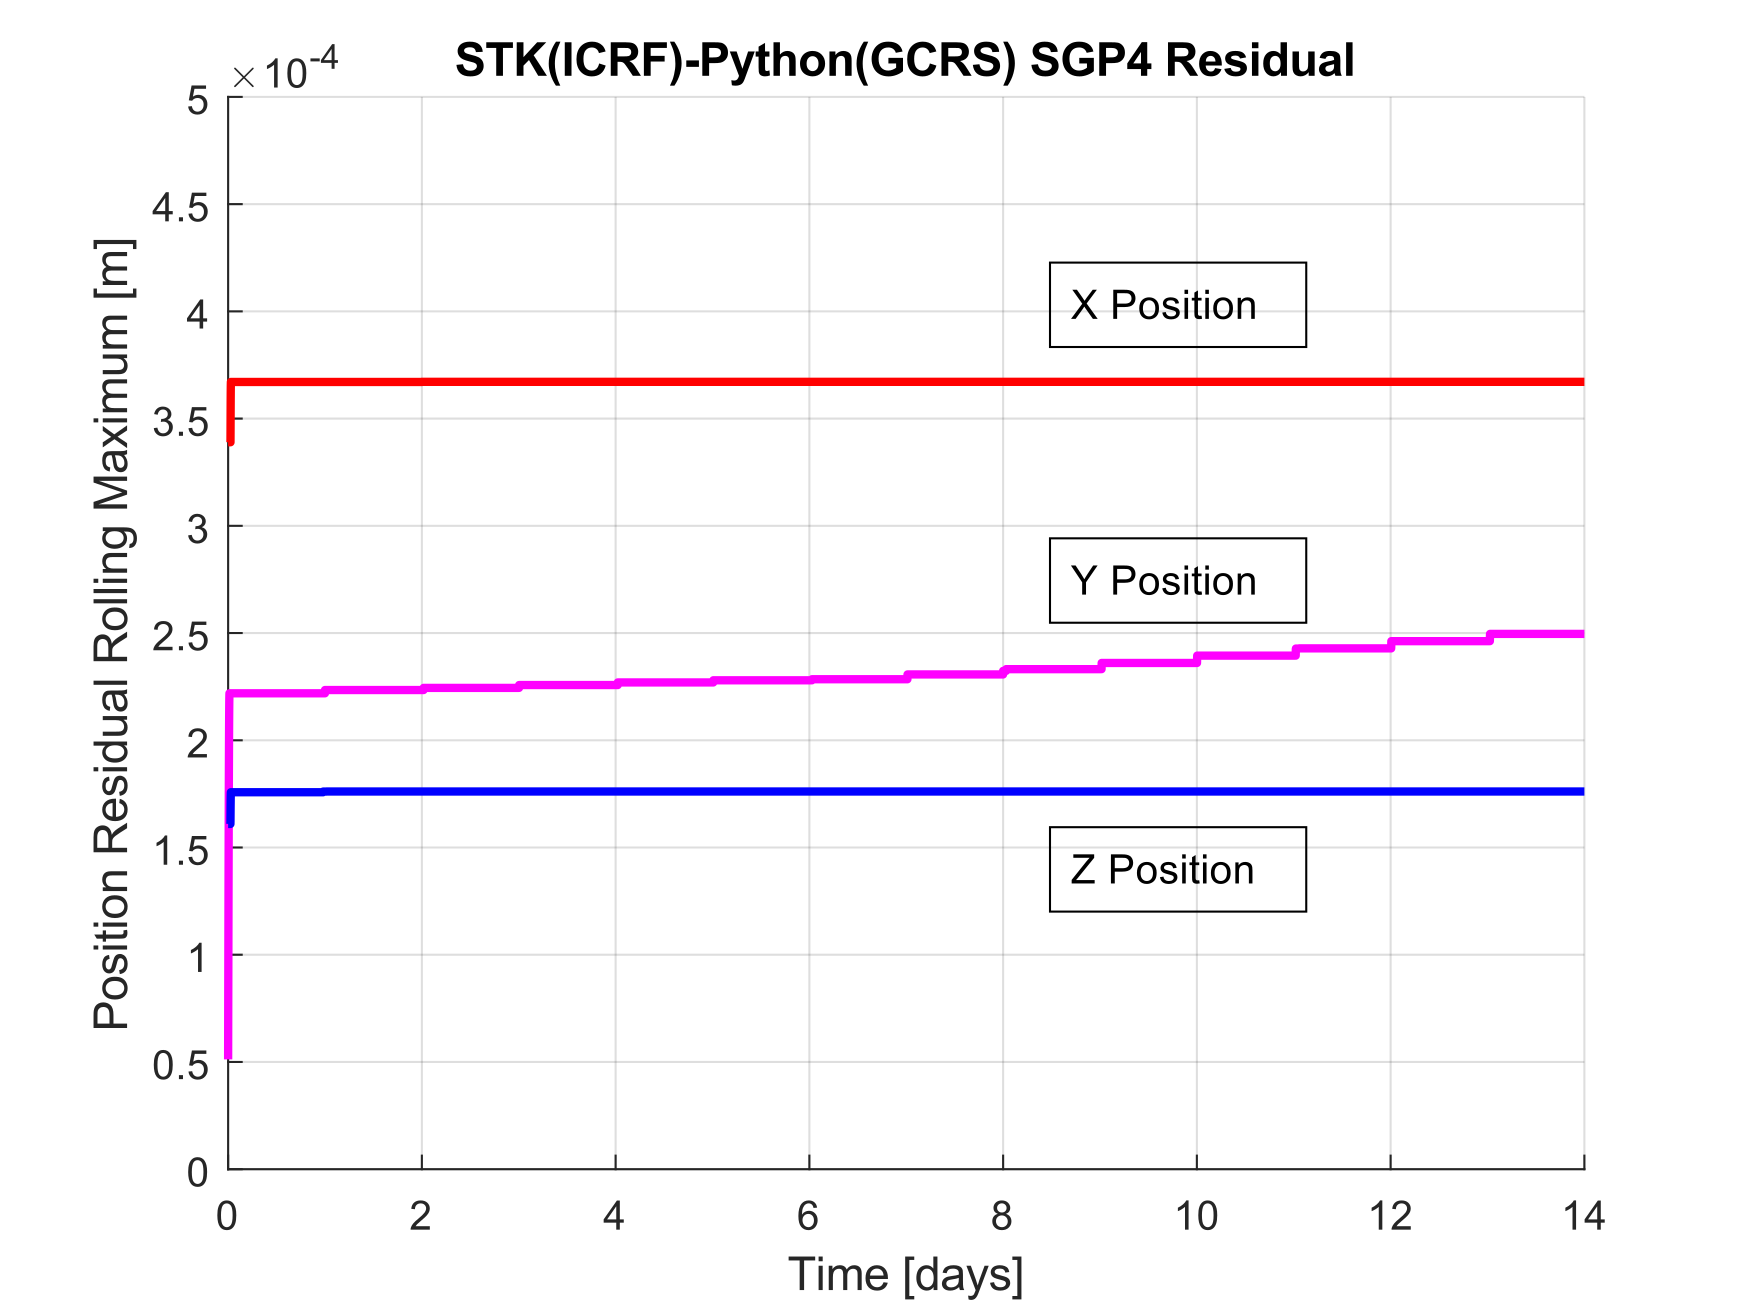
\includegraphics[width=0.7\textwidth]{STK_PY_residual-2.png} 
    \caption{Residual Difference \gls{stk} vs. Python}
    \label{fig:stk_py} 
\end{figure}

It is very easy to generate Ephemeris data. What is difficult is validating it.
The benchmark for validation is \gls{stk} since it has its own SGP4 ephemeris
generation capabilities. If operators did not use POPS, their best alternative
would be to set up scenarios manually in \gls{stk}. As such, using it as ground
truth is valid in this case. Both \gls{stk} and the \gls{pops} implementation
of SGP4 us the same source8: Revisiting Spacetrack Report \#39. As such, they
should provide the same results. One difference to note is that \gls{stk} uses
the \gls{icrf} \gls{eci} coordinate system but the propagator service uses
\gls{gcrf}.  This difference is acceptable since these reference frames are
approximately identical10. The procedure for validating the Propagator service
was first to select a \gls{tle}, a time range, a time step, and a coordinate
system.  Next was to generate Ephemerides from \gls{stk} and the propagation
service.  Finally, the results were compared. One such comparison can be seen
in Figure~\ref{fig:stk_py}. Here, the peak position residual was 0.37mm for the position along
the x-axis. The main purpose of this exercise is to ensure that the Python
libraries are being used correctly and that their output data is acceptable.
From this result, it is clear that the methods are identical and the difference
was most likely due to slight implementation differences. 

Another responsibility of the Propagator service is to determine a list of
passes for a given ephemeris. Having an entire ephemeris may be cumbersome for
some calculations so it makes sense to split a whole ephemeris into multiple
components. A `pass' is of course a completely general term so in this context
it is defined as the period between south-to-north hemisphere crossings as this
definition was chosen because it is easy to calculate an equator crossing. This
is where the z-position of a spacecraft goes from negative to positive.
\hl{See algorithm ?? for a discussion on how crossings are found}.

Part of the benefit of having the Propagator as its own service is that if a
more accurate algorithm is desired for orbital propagation, only the Propagator
service needs to be changed and the rest of \gls{pops} can be left as is.


\subsection{Access Time Utilities}

The ATU service provides the basic building blocks for
constraining observation opportunities. These can be added to depending on a
mission’s need. The \gls{atu} service currently supports calculating: ground station
access times, swath generation, horizon swath generation, and polygon
intersection with a swath. These will be discussed in detail in their own
section.  



\section{Mission Model}
 
The Mission Model service is the service that contains the main logic for most
of \gls{pops}'s functionality and front-end \gls{gui}. When a user interacts
with \gls{pops}, they are interacting with the Mission Model service. As such,
it is quite large and has a number of responsibilities. Some of them are:

\begin{outline} 
    \1 Database management,
    \1 Displaying an interactable front-End User Interface,
    \1 Earth Visualization,
    \1 Plan Configuration, and
    \1 Scheduling.
\end{outline}


\begin{figure}[h]
    \centering
    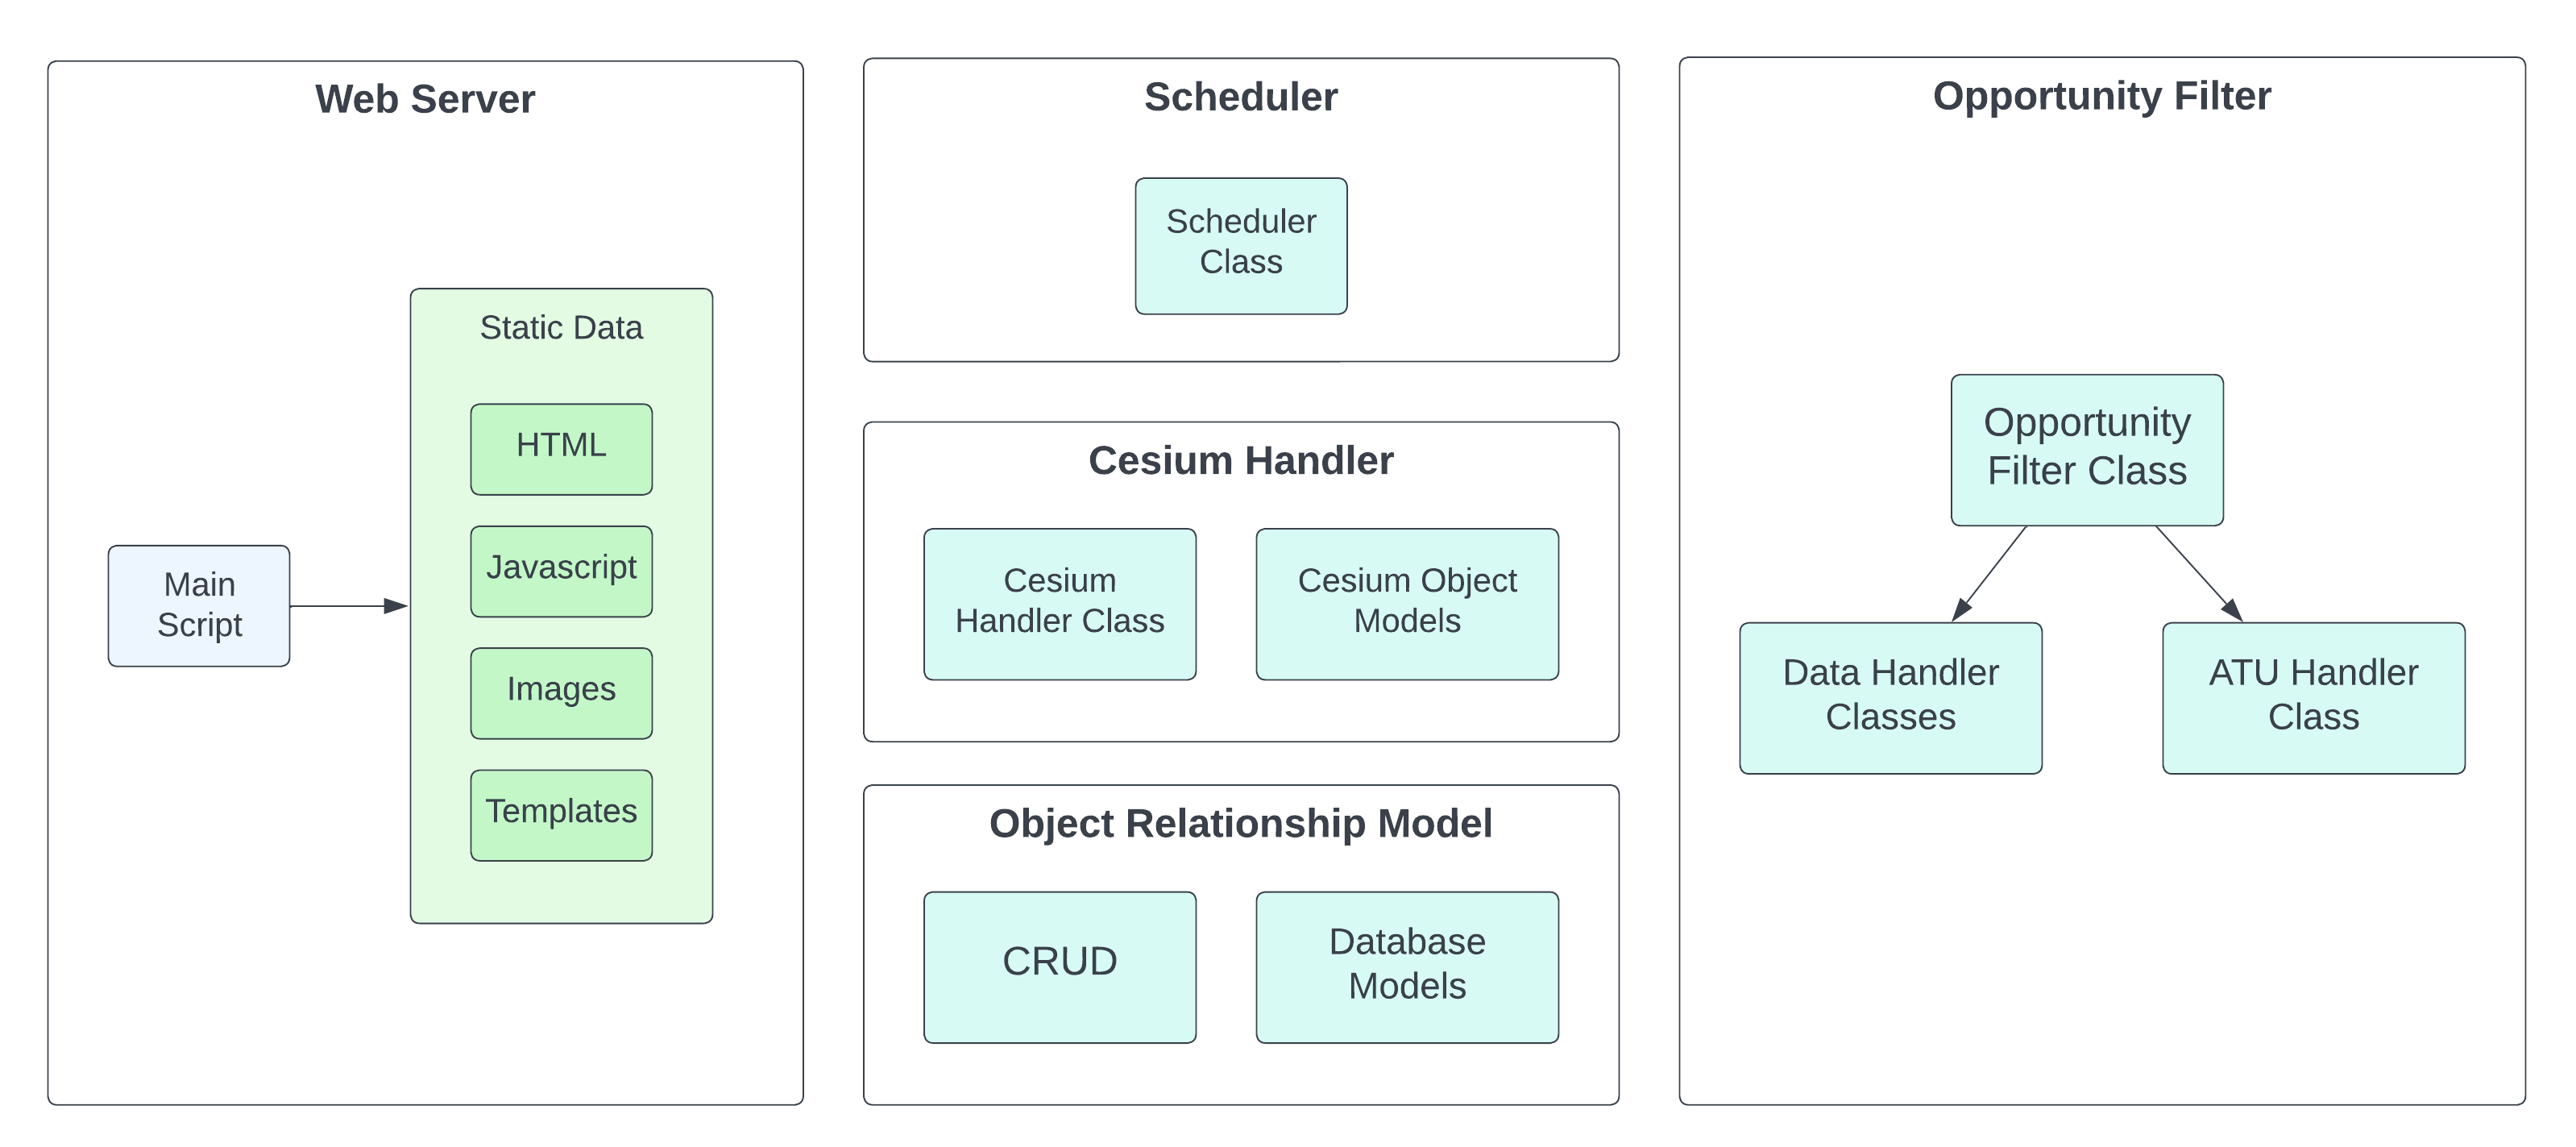
\includegraphics[width=0.7\textwidth]{Mission Model.png} 
    \caption{High Level Structure of Mission Model Service}
    \label{fig:mission_model} 
\end{figure}

A high-level overview of the Mission Model service can be seen in
Figure~\ref{fig:mission_model}. There are many components but we will go
through them one by one.

\subsection{Main} 

The main Python script acts as the base for the entire Mission Model service.
Its purpose is to, among other things, set up the web server, load environment
variables, instantiate the handler classes, and associate API calls with their
callback functions. Setting up the web server is the same as with any other
service. The environment variables range from server metadata to addresses of
other containers. There are a number of utility classes that handle various
aspects of \gls{pops}. These are the: scheduler, \gls{atu} handler, data
handler, and opportunity filter classes. They will be discussed in the
following sections. The most important part of the main service is defining API
calls. If a user wishes to interact with \gls{pops}, they must enter a link on
the their browser, that information is then sent to the web server, and a
callback function in the Mission Model service is called. It is the Mission
Models responsibility to consolidate information, whether that be from the
database, through HTML templates, or new information that must be calculated.
The Mission Model service does very few actual calcualtions, its only purpose
is to organize information and call functions as necessary to serve a request.
Currently, the main service is large and difficult to navigate because of its
size. In the future, it will be refactored to a number of sub-scripts that
handle specific functionality in the service.

\subsection{Object Relationship Mapping}

The Database is its own service but the Mission Model is currently the only
service that interacts with it. It does so by using an \gls{orm}. An \gls{orm}
is a method of modeling a relational database through an object-oriented
language. For our purposes, the \gls{orm} serves two functions, it describes
how the data is being stored in the database and it describes how we can
interact with the database programmatically. For \gls{pops}, we are using an
open-source \gls{orm} library. It handles the low-level functionality and
allows us to focus on what is unique about \gls{pops} rather than databases in
general. For example, there is no need to develop our own methods of
formulating \gls{sql} queries or parsing the ouptut data once it is retrieved. 

To set up the \gls{orm} for \gls{pops} we need at least two scrips, a models
file and a \gls{crud} file. The models file defines explicitely how tables are
layed out in the database through Python classes. Information such as: what
tables there are, what columns are in each table, what keys are included with a
table, and what relationships there are between tables. If a change is made to
the database, it must be reflected manually in the models file and vice-versa.
The \gls{crud} file, as its name suggests, allows us to interact the database.
It is a library of functions that allows a developer to formulate \gls{sql}
queries at a high level with Python syntax. The \gls{crud} file also relies on
the classes from the models file to refer to tables. For example, if we wished
to retrieve a satellite with a particular id from the \texttt{Satellites}
table, we would create a new function in the crud file with a descriptive name
such as \texttt{get\_satellite\_by\_id(sat\_id)}. Within this function we would
construct a query that searches the \texttt{Satellites} table for a row whose
id column, \texttt{Satellites.id}, matches the input id, \texttt{sat\_id}. The
\gls{orm} gives a developer a great deal of flexibility when formulating
queries or inputting data and makes interacting with the database easy to
understand and easy to expand.


\subsection{Static Data}

For the webserver to function there is a large amount of static data that must
be stored on the server and that must be retrieved when necessary. This may be
\gls{html} files, \gls{html} templates, JavaScript files, \gls{css}
stylesheets, and images.

Webpages are not generated completely programmatically. Either the \gls{html}
for these pages are written in advance and loaded directly upon being requested
or, they are assembled from HTML templates and configured depending on input
parameters given by the user or by what data is available at that time. Writing
out the HTML for a webpage in its entirety is acceptable for situations where
nothing changes on the webpage and everything should be left as is. This is the
case for high-level menus and settings pages. If anyhting else is required,
\gls{html} templates should be used. HTML templates allow for a great deal of
configurability when loading webpages. They can range from simple text
replacement to loading other templates. Some template engines even allow for
some programmatic features within the template itself such as looping, if/else
statements, or even custom functions.

Generally, as a design decision, as much of the underlying logic for \gls{pops}
has been limited to Python. The main reason for this is to consolidate the
logic to one language. Unfortunately for web development, Javascript and
\gls{css} are unavoidable and must be used as necessary. When they are used
they can be added directly to an HTML document or template but this is
generally not the best way. Having different scripts or different styles placed
haphazardly in the codebase gets messy quickly and may lead to code duplication
or even conflicting functions. To combat this, JavaScript and \gls{css} files
are stored separately and then statically referenced in the \gls{html} file
they apply to. By consolidating these files, it is much easier to organize and
reference them as necessary. 


\subsection{Data Handlers}\label{sec:data_handler}

For \gls{pops}, there is a great deal of data and many different ways that the
data can be formatted in. In an attempt to generalize the data and make them
easier for a developer to work with, several Data Handler classes have been
created to handle data format conversions and to provide helper functions. 

\subsubsection{Ephemeris Class}

Ephemerides are the most important collections of data as they are used as a
basis to calculate most other data. As such, they are referenced many times and
have a number of different formats. To illustrate what is meant by different
data formats, let us briefly jump into some specifics. There are four different
areas where Ephemerides are referenced: the Propagator service, the \gls{ATU}
service, the Cesium Viewer, and the database.




\subsection{Access Time Utilities Handler}

\subsection{Opportunity Filter}

\subsection{3D Earth Visualization}

One of the required components of \gls{pops} is a graphical 3D Earth viewer.
It goes without saying that having a spatial understanding of a mission is
absolutely necessary when performing mission planning. Only so much information
can be imparted through text.

\begin{figure}[h]
    \centering
    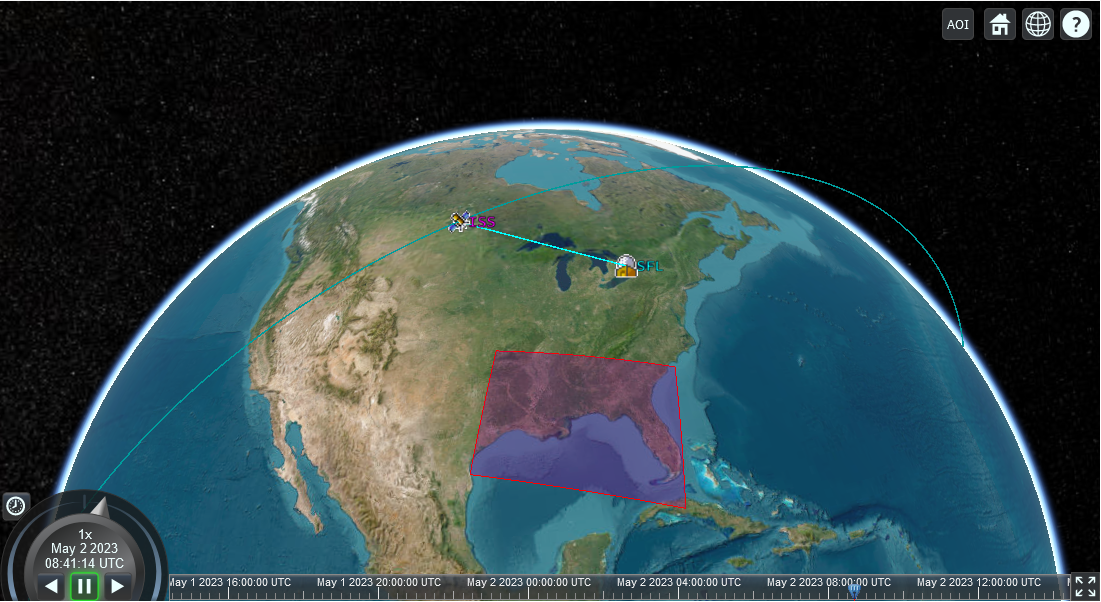
\includegraphics[width=0.9\textwidth]{Cesium_Example_Image.png} 
    \caption{Cesium Example Scenario with Example Entities}
\label{fig:example_cesium}
\end{figure}

To support this functionality, \gls{pops} makes use of the open-source CesiumJS
library. CesiumJS can display time-dynamic, geospatial information on a
webpage. CesiumJS itself is free to use and provides all of the core
functionality that is necessary for \gls{pops}. There also exists a proprietary
library, CesiumION, which provides out-of-the-box 3D terrain data and
proprietary Earth imagery. Thankfully this kind of information is superflous
for orbit operations planning. At most, all that is needed is a rough
understanding of the Earth's geography and that is sufficient. For this reason,
\gls{pops} does not provide terrain information and uses a free tile map
provider. Since \gls{pops} is only using the free version, we will refer to
CesiumJS as just Cesium for brevity. 

It should be noted that Cesium is only meant to display information to the user
and intended to be a tool that performs any calculations. All data is generated
through other means and then converted into a format that Cesium can display.
The reason for this is that, since Cesium is such a large tool, it is difficult
to validate in great depth because it is not clear what assumptions are being
made at what level. So, as long as the entities being displayed by Cesium are
qualitatively correct then that is sufficient.

An example scenario generated by \gls{pops} can be seen in
Figure~\ref{fig:example_cesium}. There, a few key elements of a Cesium viewer
are visible. On the bottom, there is a timeline with some controls. A user can
change the time of the scenario as they like and the scenario will update
dynamically. This is very similar to tools such as \gls{stk} so an operator
will be used to working in this way. In the centre the Earth can be seen with
the camera hovering over North America.  The camera can be moved with the mouse
or can be fixed to a particular position and orientation programmatically.
Some entities have been added to the scenario. At the bottom, a polygon has
been drawn on the Earth. A very useful feature of Cesium is that polygons can
be defined with vertices and edges clamped to the WGS84 Ellipsoid. That is,
vertices are placed on the Ellipsoid and edges are not straight lines but great
ellipse arcs. This saves a great deal of calculations and code that must be
maintained. Above the polygon, can be seen a satellite, the \gls{iss}, and a
ground station, the \gls{sfl}. The ground station is fixed but the satellite
orbits the Earth and changes position as the time changes in the scenario. The
satellite's path is given by the teal line. 

Every object in the Cesium viewer is treated as a single entity. There are two
ways entities may be added, updated, or removed from a Cesium viewer. Either,
through JavaScript, where a developer creates new objects programmatically, or,
through a custom \gls{json} format called \gls{czml}. Though Cesium has an
extensive client-side \gls{api}, \gls{czml} allows the cesium scenario to be
generated from data rather than from custom code. Most of the underlying data
is calculated through Python scripts so it is more appealing to have an
interface that generates \gls{czml} data rather than having additional
JavaScript. Also, by generating \gls{czml}, logic is not split between the
backend Python code and front-end Javascript. In this way, the Python drives
what is being shown in the Cesium viewer. \gls{czml} also allows for
incrementally streaming data to a client. That is, not all of a scenario needs
to be available immediately once a scenario is loaded. Rather, \gls{czml} data
can be sent in a number of packets, and can be added as they become available.

To set up a viewer, some JavaScript is needed. A placeholder is placed
somewhere in the webpage hosting the viewer then the JavaScript searches for
that placeholder and inserts all of the necessary data to generate the viewer.
Some parameters need to be set for the viewer such as: the imagery provider,
rendering modes, lighting, display options, or toolbar buttons. Once a viewer
is created, it runs until it or the page is changed.  To facilitate
communication between the Cesium viewer and the Python backend, a websocket is
created as they allow for bi-directional communication. 

\subsection{Cesium Models}

Even though we are using Cesium as our 3D Earth visualization tool, a
substantial amound of development must be done to properly configure and manage
what is being shown on the viewer. Before discussing how a Cesium viewer is
managed, it would be useful to first go over what can be displayed currenlty
with \gls{pops}, the Cesium Models. These model classes are not like the ones
made for \gls{orm}, rather these models have two responsibilities. They must
keep some metadata about a Cesium object and they must contain a method that
generates a valid \gls{czml} packet.  A \gls{uml} diagram that summarizes all
of the currently implemented Cesium models can be seen in
Figure~\ref{fig:cesium_models}. It should be noted that the diagram does not
contain an exhaustive list of all of the member variables for each class;
rather, it contains the most important variables.  Each model contains some
information about the object that does not change once it is created. For
example a satellite object will not change which satellite it references once
it's created. 

\begin{figure} \centering
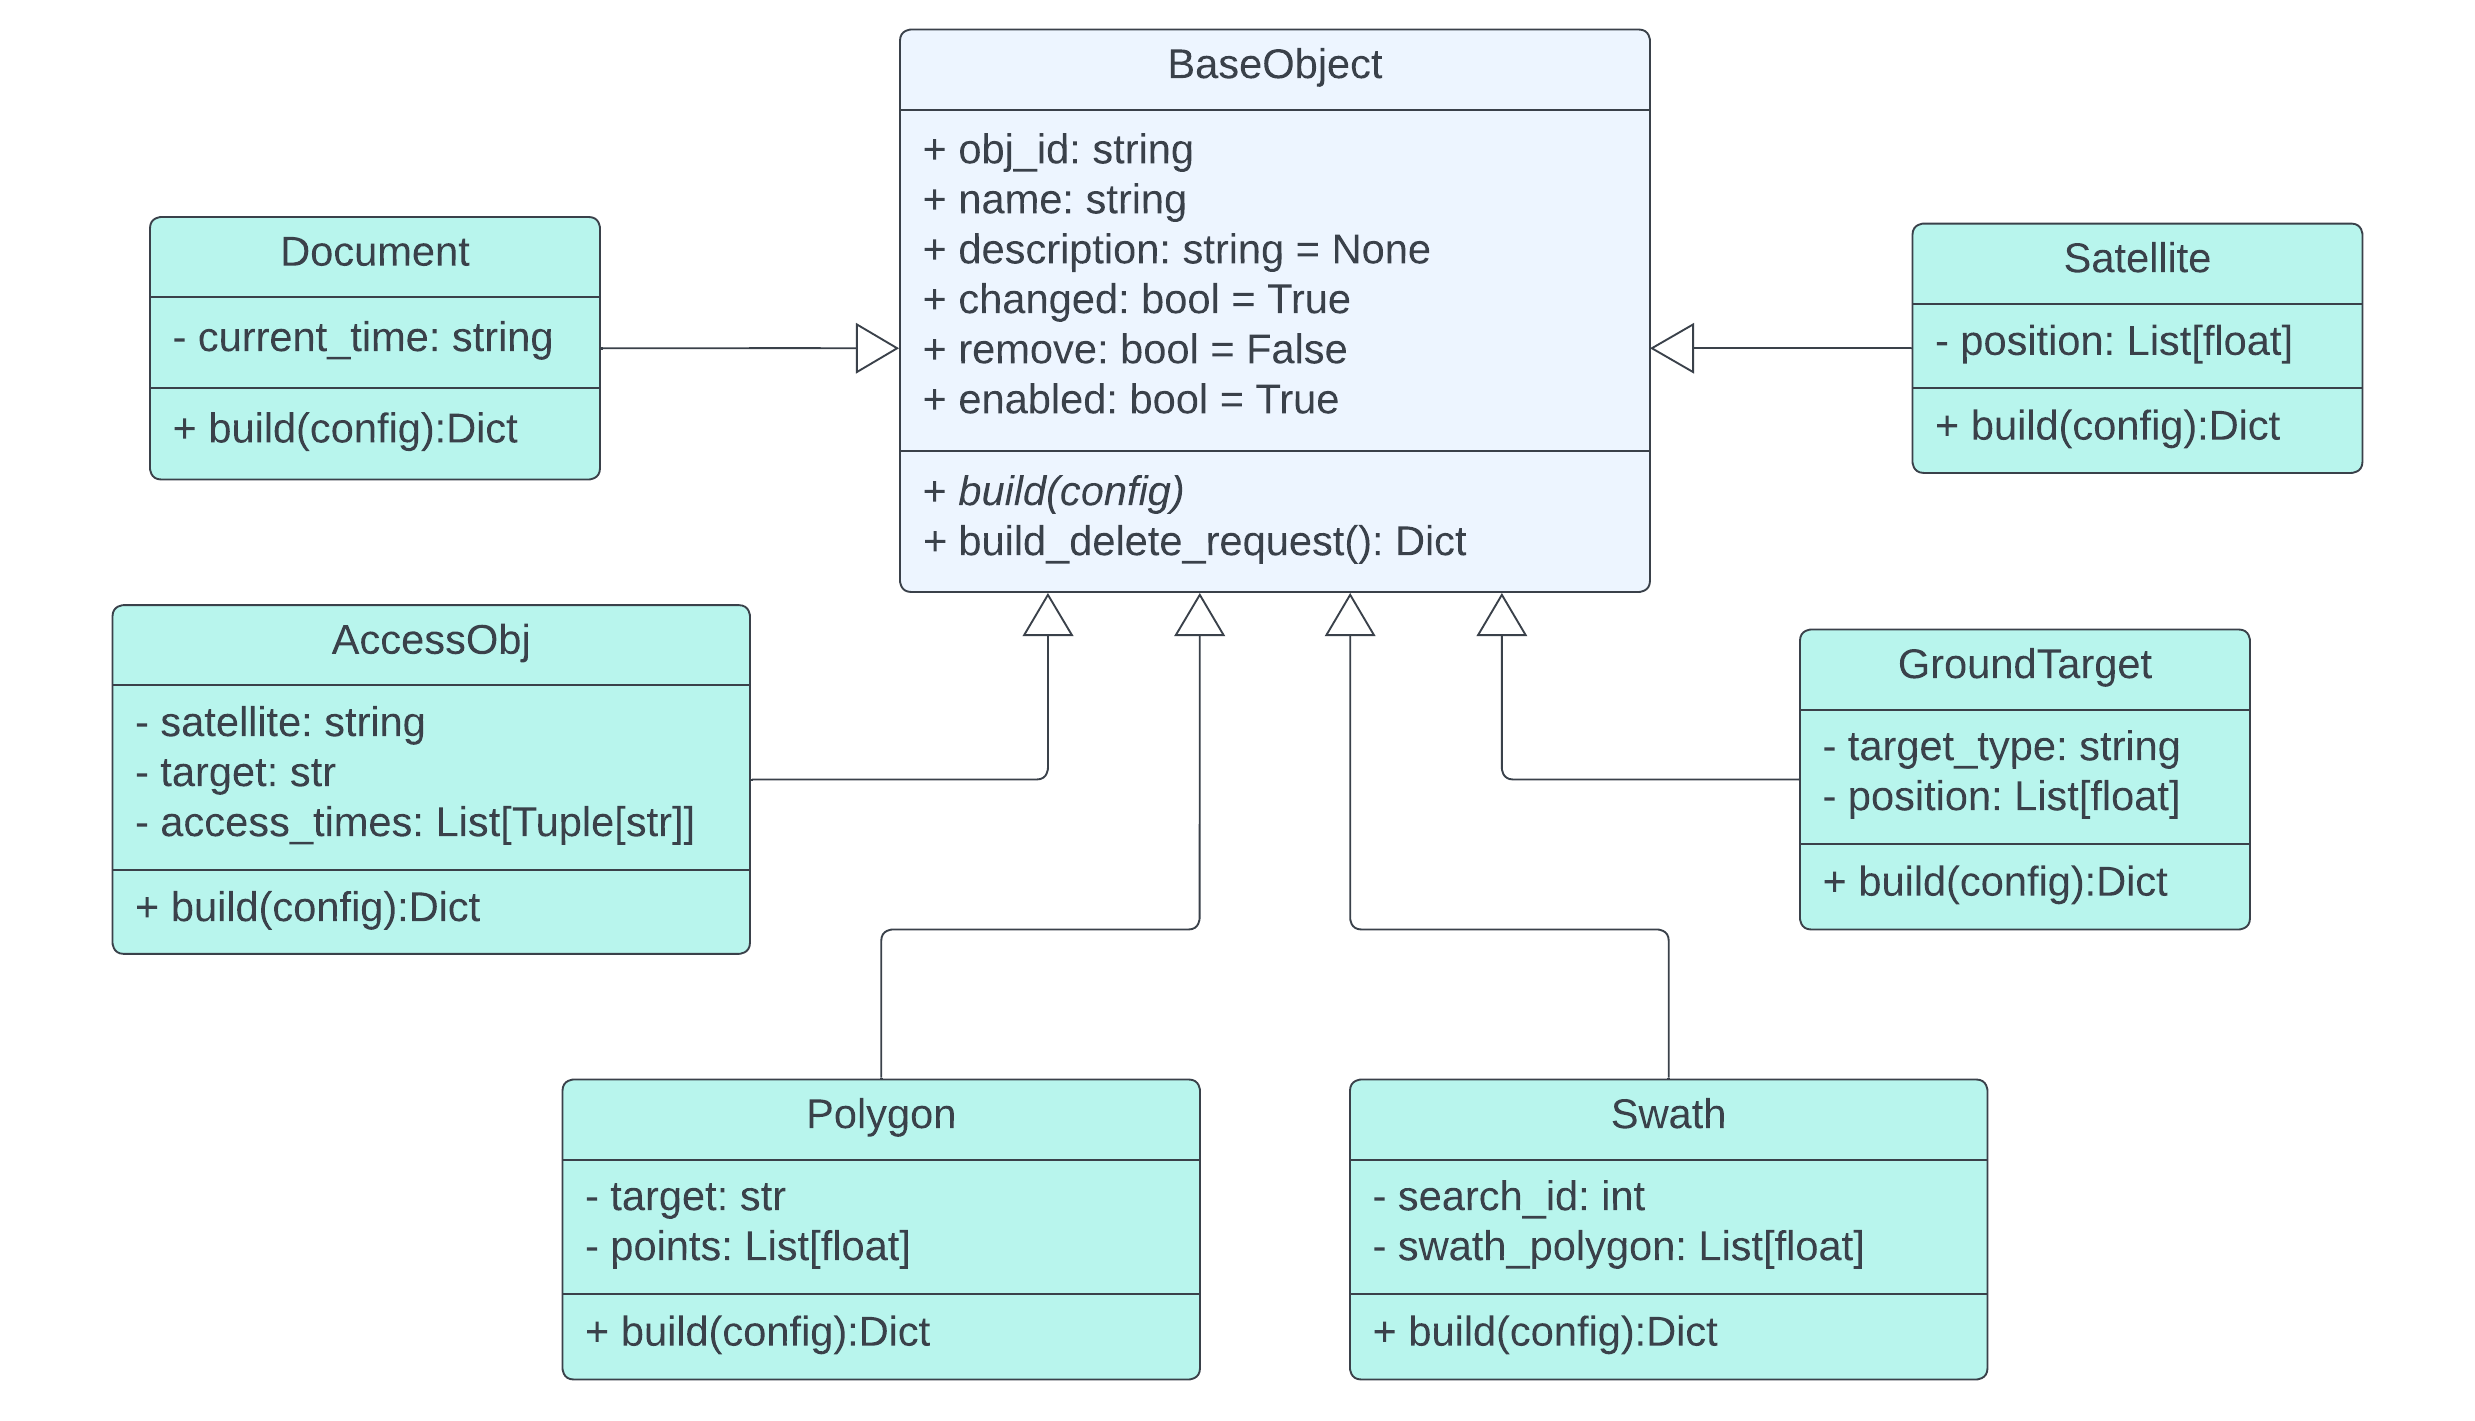
\includegraphics[width=0.9\textwidth]{Cesium_Models.png} \caption{Cesium Models
UML} \label{fig:cesium_models} \end{figure}

To begin, there is a \texttt{BaseObject} class which serves as a general parent
class to all Cesium objects. It defines member variables that are common to all
objects. Properties such as the object's unique ID, its display name, and its
description. In addition there are three flags that describe the `state' of the
object: \texttt{changed}, \texttt{remove}, and \texttt{enabled}. If the
\texttt{changed} flag is set, this indicates to the Cesium Handler class that a
new \gls{czml} should be generated for that object. By default, every time an
object is created, the \texttt{changed} flag should be set. Once \gls{czml} is
generated and uploaded to the viewer, this flag is reset. If the
\texttt{remove} flag is set, this object should be removed from the Cesium
viewer, and once this is done, the object should be deleted. Lastly,
\texttt{enabled} hides Cesium Entities without unloading them from the viewer.
Each sub-class has its own implementation of the \texttt{build()} method, since
building a \gls{czml} object is unique to that object.
\texttt{build\_delete\_request()} is common to all Cesium objects since the
request only contains the object's ID. The currently supported Cesium models
are as follows:

\begin{description} 

    \item[Document] Each Cesium scenario must have one and only one
	\texttt{Document} object as it specifies general scenario data such as:
	what is the scenario's time range, what is the current time in the
	scenario, or what is the scenario's timestep. Once this object is set
	for a scenario, it does not need to be set again unless the current
	time should be changed.

    \item[Satellite] Satellites are represented through a small \gls{png} image
	called a `billboard'. They are given a descriptive label that maintains
	a fixed position with respect to the satellites position. To have the
	satellite move over time within the scenario, an ephemeris must be
	included in the object. This ephemeris must conform to a particular
	format and this conversion is handled by the Ephemeris data handler
	discussed in Section \ref{sec:data_handler}. Lastly, a satellite is
	given a path to visualize to the user, where the satellite will and has
	been for some period in the future and the past.

    \item[Ground Target] Ground Targets are essentially the same as Satellite
	objects but, in this case, they are given only one position for the
	entirety of the scenario. Ground Targets can be \glspl{aoi}, ground
	stations or any other stationary ground object.

    \item[Access Object] It is useful to display when a satellite has access to
	a ground target. This is accomplished through drawing a polylline
	between the satellite and the ground target for times where they have
	access to each other. One useful feature of \gls{czml} is that we can
	reference the position of other object by reference to their ID. This
	saves us from having to load a satellite ephemeris into the object to
	describe the position of the satellite. \gls{czml} also allows us to
	specify when an object should or should not be visible by specifying
	intervals of visibility. When an \texttt{Access Object} is created we
	must pass a list of access times such that we may define these
	intervals in the object.

\begin{figure}
    \begin{minipage}[c]{0.45\textwidth}
	\centering
	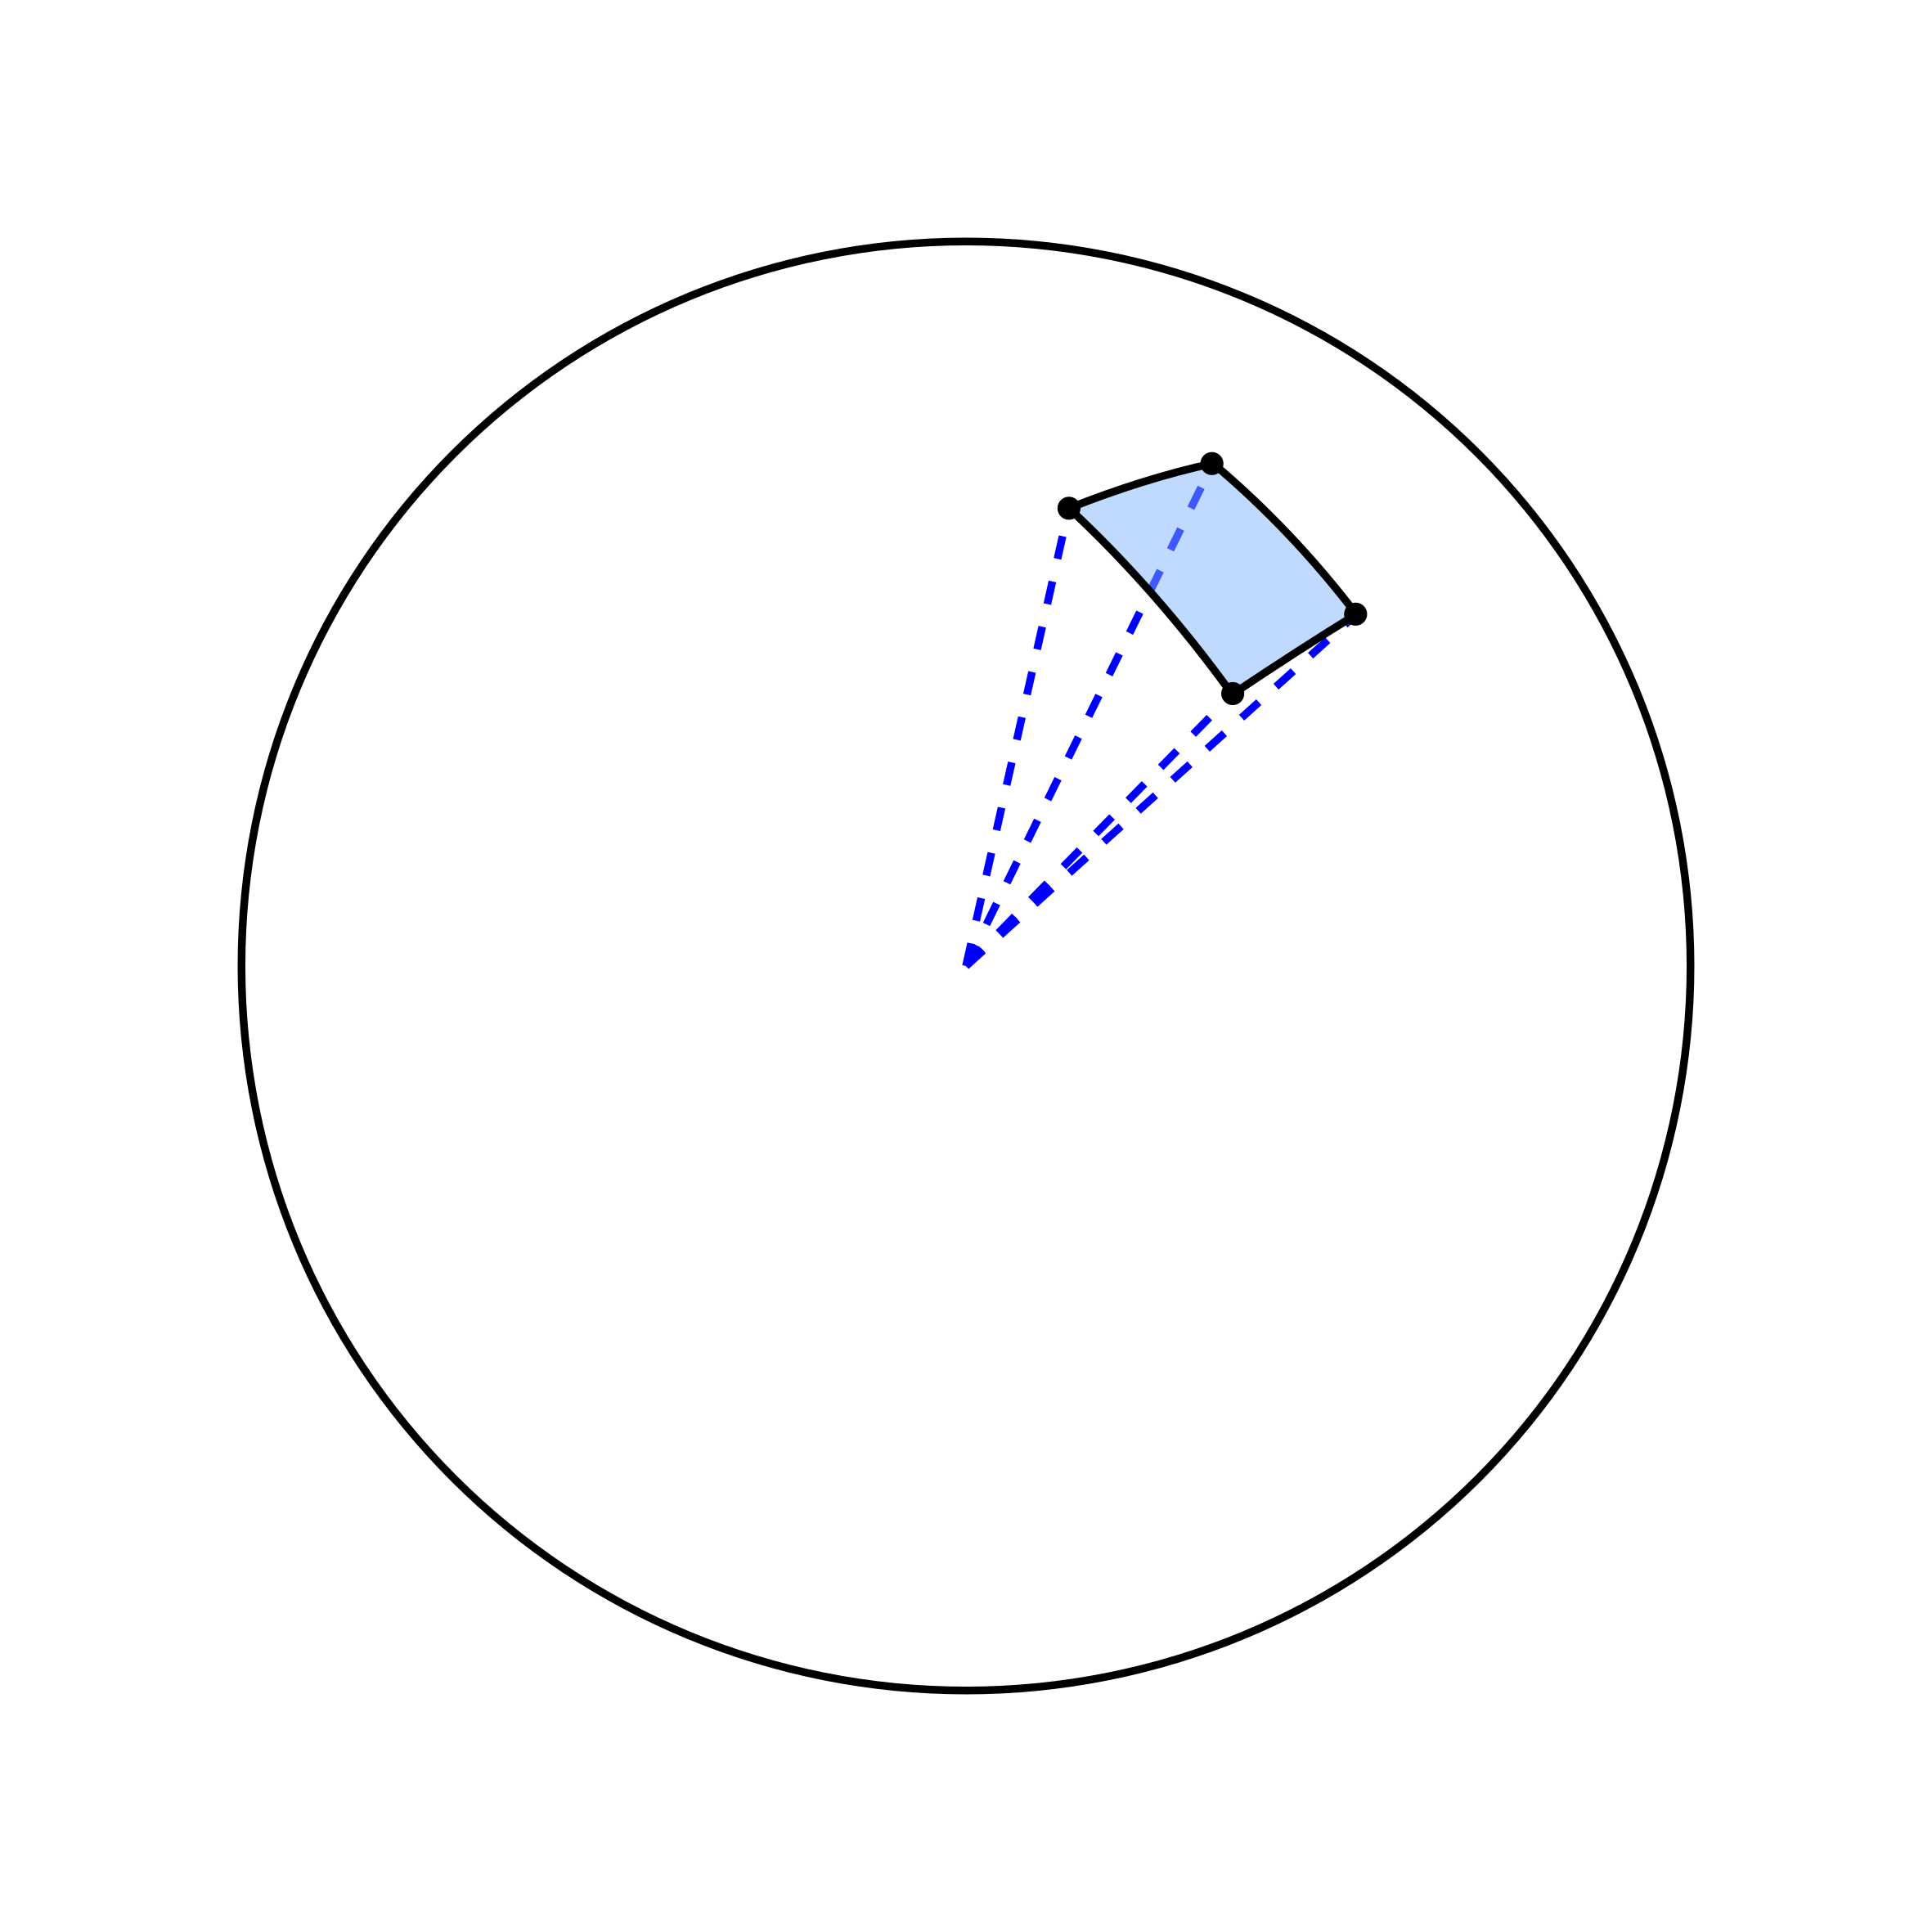
\includegraphics[width=1\textwidth]{inside-outside-2.png} 
	\caption{Smaller Area}
	\label{fig:inside_polygon_1}
    \end{minipage}
    \hfill
    \begin{minipage}[c]{0.45\textwidth}
	\centering
	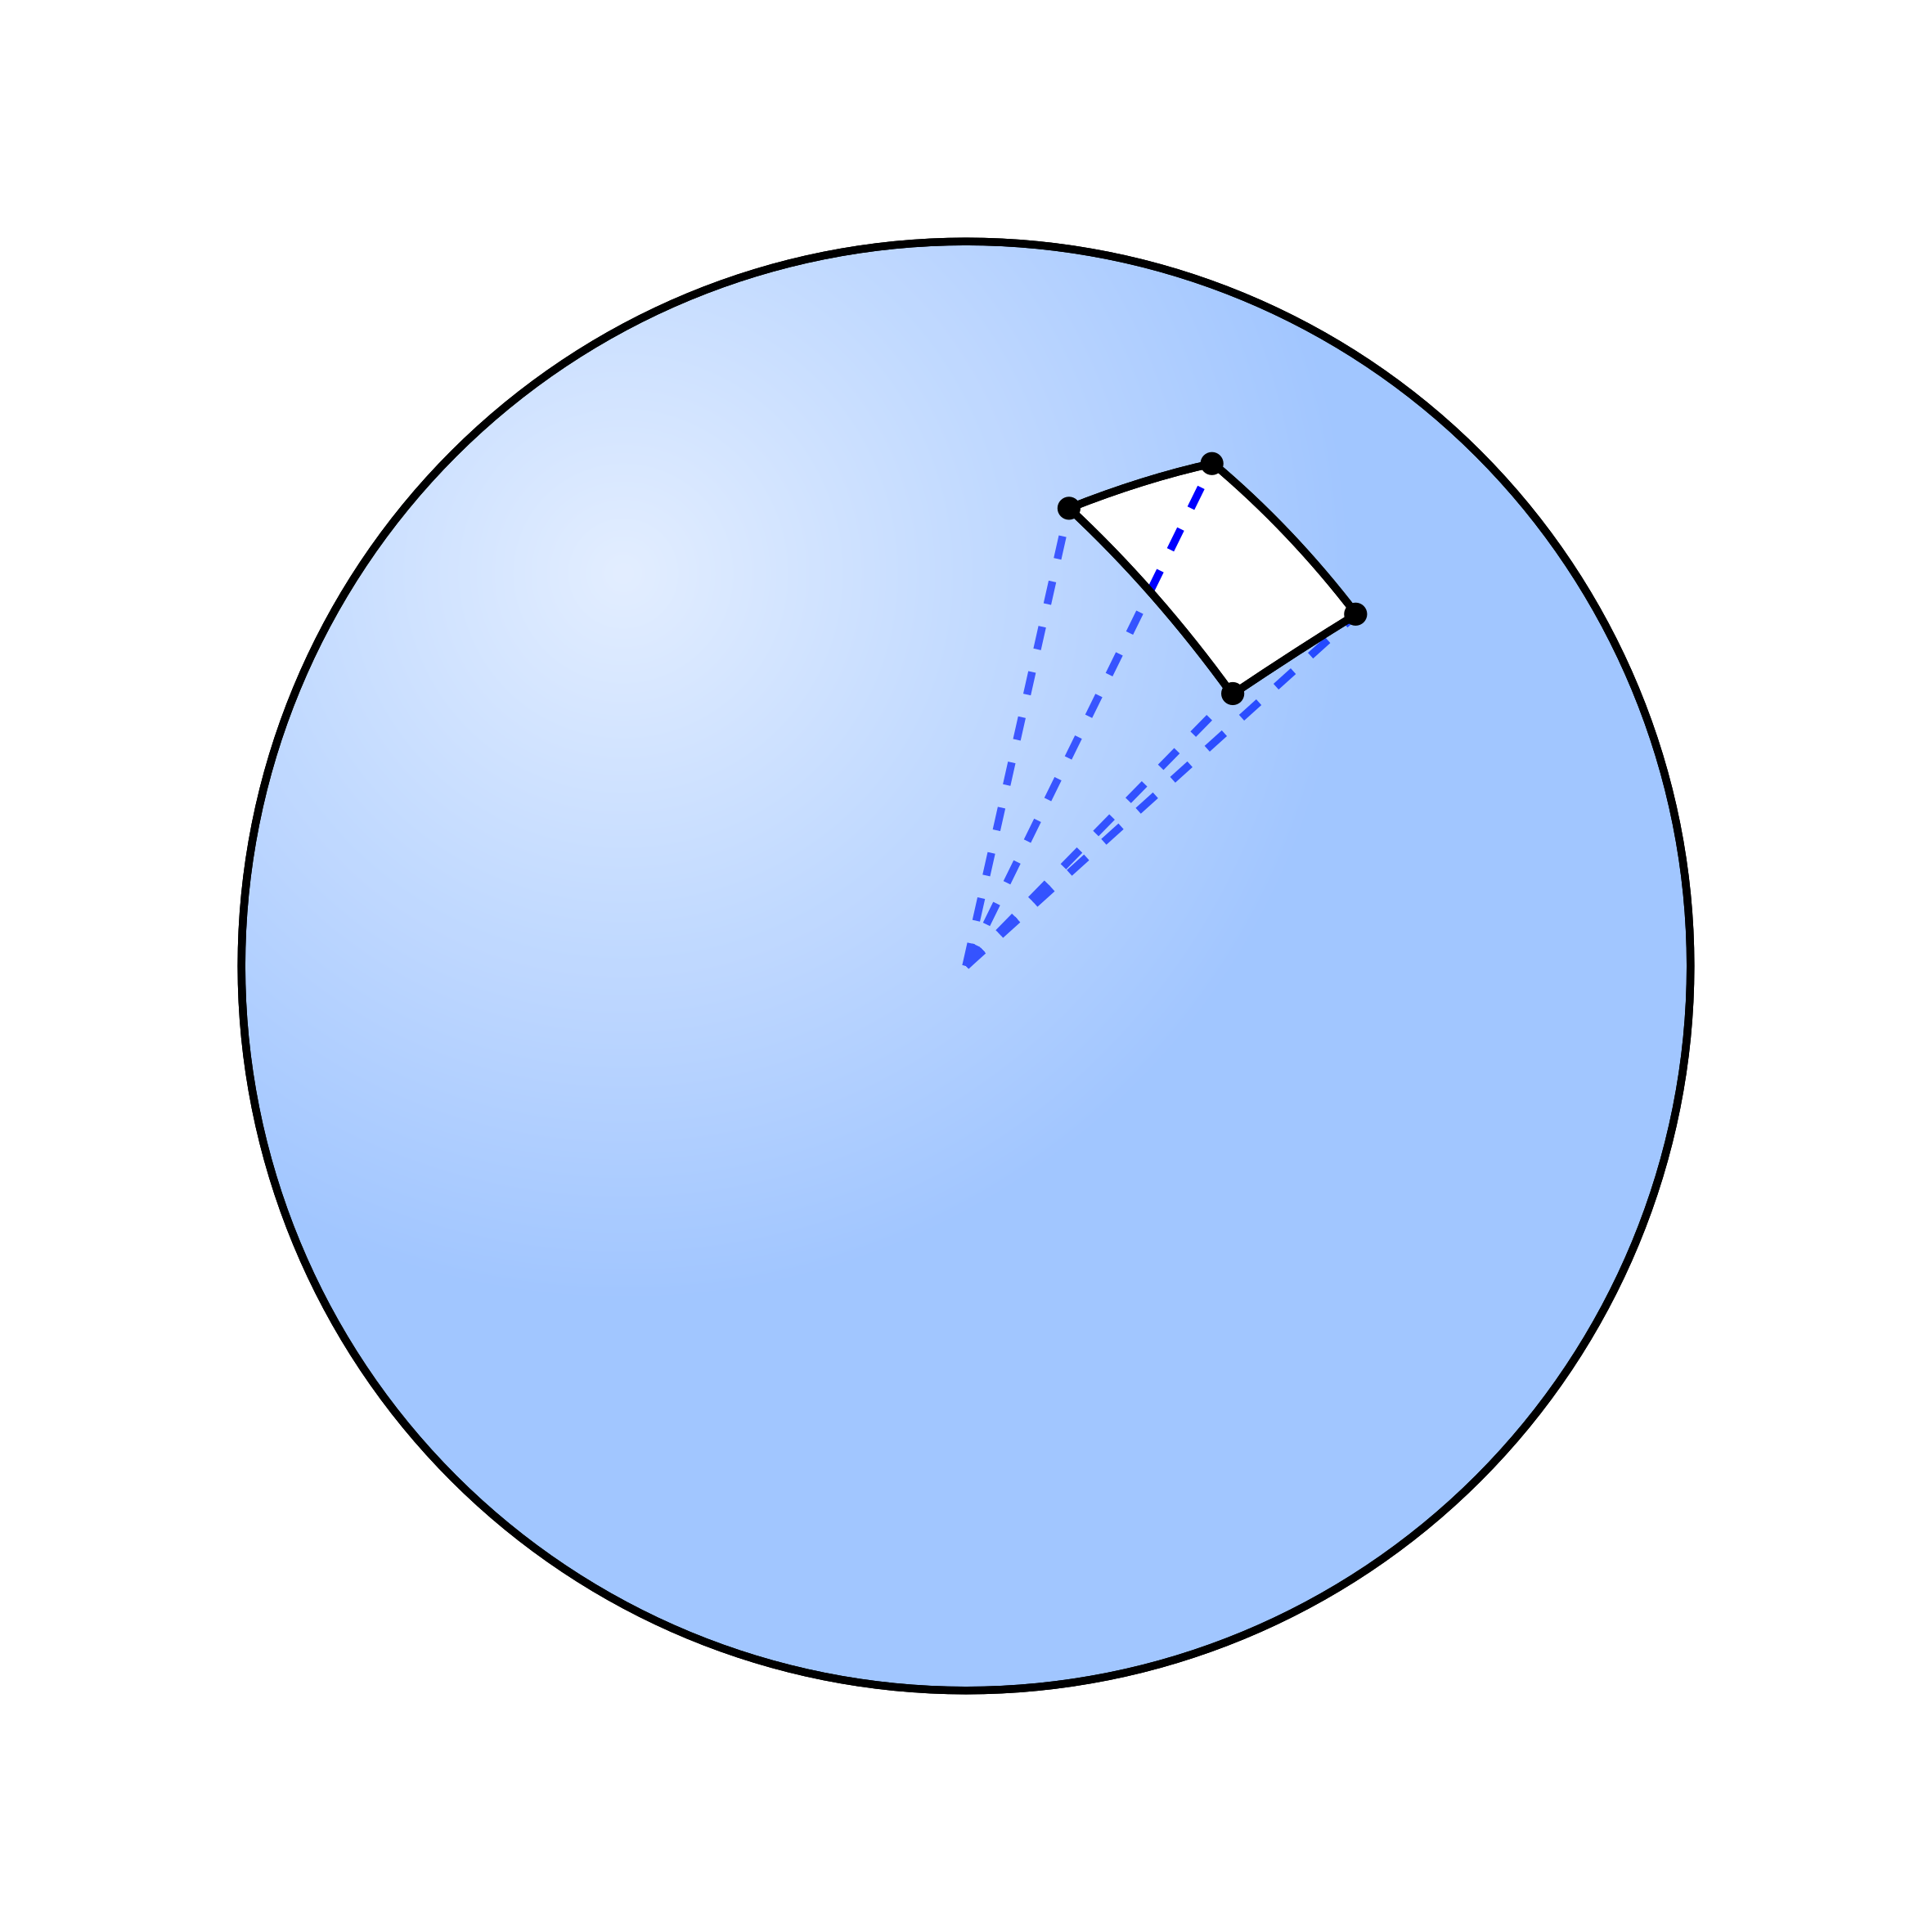
\includegraphics[width=1\textwidth]{inside-outside-1.png} 
	\caption{Wider Area}
	\label{fig:inside_polygon_2}
    \end{minipage} 
\end{figure}


    \item[Polygon] As mentioned earlier, Cesium has the ability to display
	polygons in any number of ways but, for our purposes, we are mainly
	focused on polygons clamped to the Earth's surface. The two instances
	where polygons are currently used for \gls{pops} are for Area Target
	\glspl{aoi} and for intersection polygons. The difference practically
	for these two cases is just in their colour. To draw a polygon in
	Cesium, we must provide it a list of points in Cartesian coordinates or
	in Latitude-Longitude-Altitude coordinates. For the Cartesian
	coordinates, if a point does not directly lie on the WGS84 Ellipsoid,
	Cesium will only draw the closest point on the Ellipsoid. From this
	list of points, Cesium will guess the `inside' of the polygon. Note
	that since we are drawing shapes on an Ellipsoid, the geometry is
	non-Euclidean. The inside of a polygon on a 2D plane is clear for
	polygons that do not self-intersect; it is simply the the region that
	is enclosed by all of the sides of the polygon. For an Ellipse any
	point can be enclosed. See an example of this in Figures
	\ref{fig:inside_polygon_1} and \ref{fig:inside_polygon_2}. Both have
	identical polygons where there are 4 vertices on the Ellipsoid and
	their edges are the same. There is now a question of what forms the
	inside of the polygon as this can be the larger area or the smaller
	area. There are a number of ways this can be addressed. One way is to
	specify the points on the polygon in a clockwise or counter clockwise
	order. Then the internal area will be whatever conforms to this
	ordering. Another way would be to specify one or more points that are
	not vertices but rather example points that lie within the polygon. In
	this way the area of the polygon will be the set of points that contain
	the example point. For simplicity, Cesium makes a best guess at what
	the inside of a polygon is by selecting the inside with the smaller
	area. This is sufficient for smaller polygons but for larger or more
	complicated polygons where the intended area is greater than one half
	hemisphere, determining the inside of a polygon no longer becomes clear
	and the viewer displays a garbled result. Alternatively, if there is a
	polygon which intersects itself, Cesium also becomes confused. In these
	scenarios, a large polygon must be sub-divided into sections that
	Cesium can process.

\begin{figure}
    \centering
    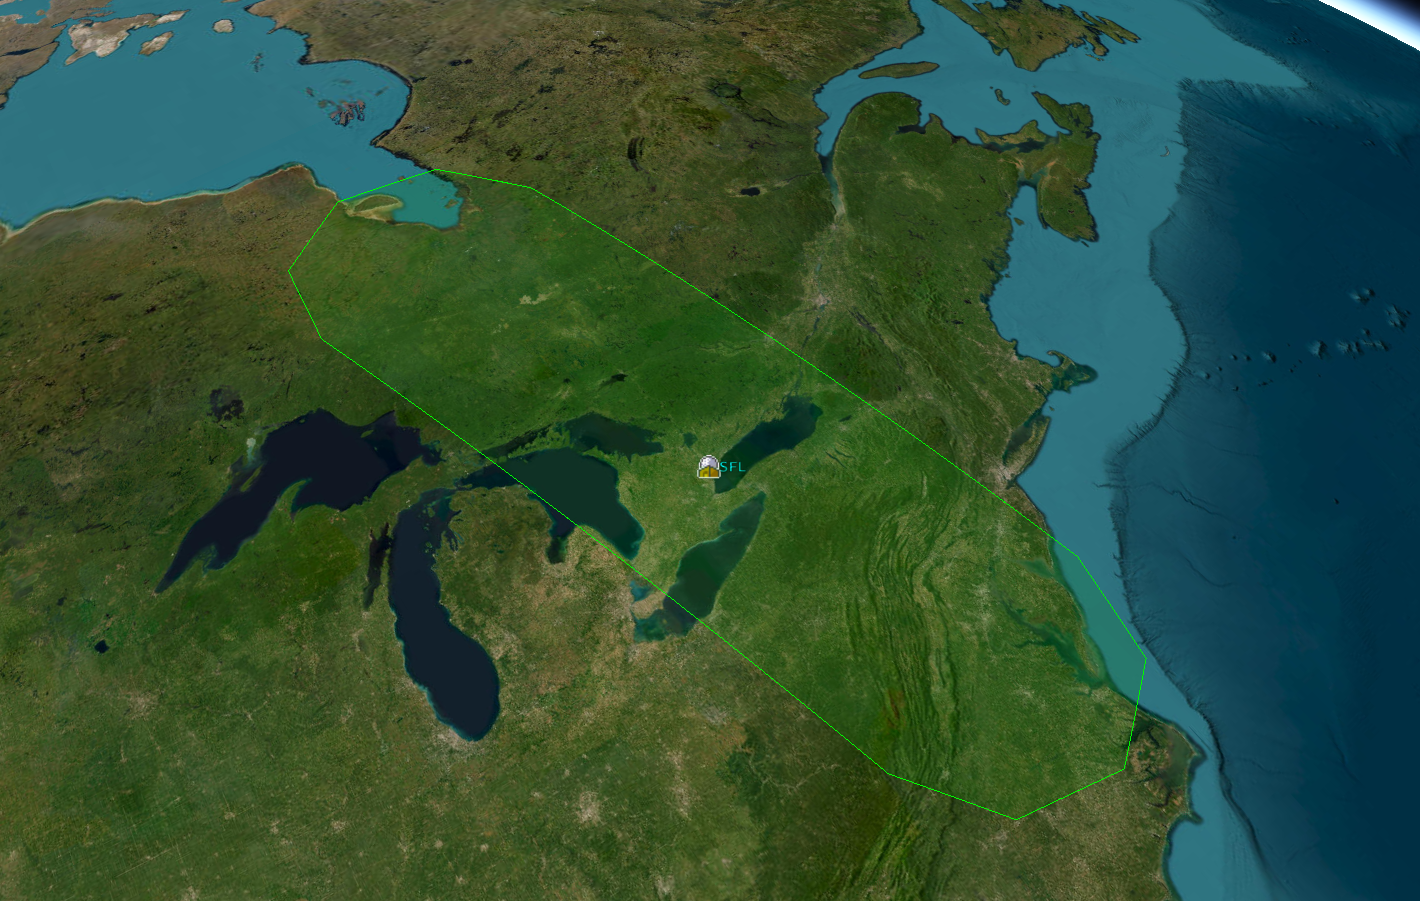
\includegraphics[width=0.9\textwidth]{Cesium_Example_Swath.png} 
    \caption{Example of a 30$^\circ$ Ground Swath}
    \label{fig:cesium_swath}
\end{figure}

    \item[Swath] The last Cesium object that is currently handled are ground or
	access swaths. The distinction here between \gls{fov} and \gls{for} is
	unimportant since both are displayed in the same way. Swaths are
	displayed with polygons but how they are generated can be tricky. From
	the \glspl{atu}, swaths are represented through two polylines that loop
	around the Earth $L_1$ and $L_2$. These represent the left and right
	boundary of the swath with respect to the velocity vector (See
	section~\ref{sec:atu}).  Typically, to display a swath all that we must
	do is reverse $L_1$ and append it to $L_2$. In this way we create a
	counter-clockwise ordered polygon that can be displayed on Cesium. But,
	if we do this for a swath that is defined for greater than one
	half-orbit Cesium will no longer be able to display the polygon because
	it cannot determine what the inside of the polygon is. Thankfully,
	swaths generally only need to displayed for times where a satellite has
	access to an \gls{aoi}. Automatically sub-dividing swaths for longer
	time ranges will be handled in future iterations of \gls{pops}.
	Combining the two swaths boundaries is mostly sufficient for display
	purposes but at the beginning and end of a constrained swath, we may
	wish to show the footprint or access region of the satellite at the
	beginning and end of the constrained swath. To do this, the \glspl{atu}
	also provide ellipse lists for each point in an Ephemeris. From this
	list, we can take the ellipsoids at the beginning and end of the
	constrained swath, take only the points that lie outside of the swath
	area, and append them to the boundary lists. That is,
	\begin{equation*} 
	    P_{swath} = L_1' + E_{start} + L_2 + E_{end}
	\end{equation*} where $P_{swath}$ is the swath polygon, $L_1'$ is $L_1$
	reversed, and $E_{start}/E_{end}$ are the ellipse points at the
	beginning and of the constrained swath. Calculating $E_{start}/E_{end}$
	is somewhat involved and is discussed in Algorithm~\ref{alg:ellipse}.
	An example of a swath can be seen in Figure~\ref{fig:cesium_swath}.

\end{description}


\subsection{Cesium Models}

Now that we have an understanding for all of the basic objects that are
supported by \gls{pops}, we may now discuss how they are combined to display
mission information to a user. For this, a Python Cesium Handler class has been
written that acts as the interface between the Python backend and the Cesium
viewer frontend. The Cesium Handler class: keeps track of the entities
currently in the Cesium viewer, keeps track of what entities have been changed
or that need to be updated, and generates new \gls{czml} data to be sent to the
viewer. When the \texttt{main} script is first run, it creates an instance of
the Cesium Handler class as a global variable. In this way it can be referenced
as needed by any api call. Some libraries do exist that perform this
functionality but \gls{pops} has enough custom entities that an equivalent
amount of development would need to be done to support them anyway.

To keep track of entities in the viewer, the Cesium Handler class has a list of
objects where each object is a Cesium Model. As such, it has all of the meta
information of the \texttt{BaseObject} as well as a method to build a
\gls{czml} packet and delete packet. By setting up Cesium objects in this way,
they can be treated completely generally by the Cesium Handler class and
metadata can be stored and referenced for every object. This metadata tracks
the status of Cesium objects and determines whether any changes need to be made
in the viewer. 

Objects can be added or removed with helper funcitons in the Cesium Handler
class. Either objects can be added directly, by creating an instance of a
Cesium Model class, then adding them to the list of objects in the Cesium
Handler or a developer can use one of the helper methods. Some situations may
require specific logic to set up a scenario. This is the case for displaying
search scenarios or adding opportunities to a viewer. Currently, there is no
way to generally display the results of a search scenario. A developer must
explicitly define what swaths, intersection polygons, or \glspl{aoi} to add. In
the future this may bemade completely general through some sophisticated but
the current method is sufficient. As with the database, opportunities are also
linked in the Cesium Handler class so that they can be referenced and enabled
or disabled as desired. This makes visualizing search scenarios much more
clear. 

To actual effect changes to the Cesium viewer, the Cesium Handler makes use of
an asynchronous approach. A user may make a change to the Viewer at any time or
they may even make many changes in quick succession and the Viewer must be able
to update correctly. Whenever a change is made to the objects list, first,
\gls{czml} packets are generated for each object whose\texttt{changed} flag is
raised. In this way czml is only sent when necessary and the viewer is not
bombarded duplicate data. These packets are then added to a queue. Then, a flag
is raised in the Cesium Handler class to signal that packets are ready to be
sent to the Cesium Viewer. Within the \texttt{main} script there is a loop that
checks for this flag. Once it is raised, the \texttt{main} service sends every
\gls{czml} packet to the viewer then verifies that the correct number of
packets were received in a return message. If the validation passes, then the
changed flag is reset for all of the objects that were processed. The reason
for using a queue is that it allows for many requests to be processed quickly
without it potentially jumbling the viewer.


\subsection{Scheduler}




\section{Database}

\gls{pops} must be able to retain information, even if it is
shut down or moved somewhere else. It is also necessary that data be stored
such that it does not sit in RAM. For this reason, an SQL database service is
included. It stores all the data necessary for \gls{pops} to function. This
includes but is not limited to satellite information, \gls{tle}s, current and
previous plans, ephemeris data, observation opportunity data, and planned
observations. Using an SQL database allows for effective data storage and
access. There are also no read or write restrictions on an SQL database so data
can be accessed simultaneously by multiple users or services.





\section{Access Time Utilities}


The Access Time Utilities are the fundamental components that enable POPS to be
a planning software. They form the basic building blocks for constraining
observation opportunities. Additional utilities can be added depending on a
mission’s need. The following sections discuss the baseline functionality that
has currently been implemented.


\subsection{Ground Access Utility}

A Ground Access is defined as the time interval during which a satellite can
establish contact with a ground station. A ground station is a point on the
Earth’s surface, identified with geodetic latitude-longitude-altitude
coordinates and an elevation mask. An elevation mask is the angle above the
horizon, at the ground station’s position, at which the satellite can be
considered visible by the ground station. Calculating the ground access for
satellites on a mission is a fundamental task in operations planning. These
time intervals dictate the opportunities for data downlink, command uplink, and
any other communication between the ground segment and satellite. 

The simplest way to compute ground access involves propagating the orbit of a
satellite and checking, at every time step, the position of the satellite
relative to the ground station and testing whether the relative position is
above the elevation mask. While this method is trustworthy and capable of
returning accurate results, its reliance on iterating over an entire satellite
orbit input typically yields a long runtime. This is particularly evident in
the case where a mission has multiple ground stations, multiple satellites, or
a short propagator timestep. The computation time drawback motivates the use of
other algorithms that can determine ground access more efficiently. 

There have been a plethora of papers published on the subject of efficiently
computing ground access over the years. Early work includes Lawton’s
development of a method for calculating ground access for low-eccentricity
satellite orbits by leveraging the Fast Fourier Transform to quickly find a
ground access11. Alfano et al.12 use another technique known as parabolic
blending for constructing the visibility function and finding ground access.
While POPS currently utilizes the simplest method for calculating ground
access, the method that is selected for future implementation is that of Han et
al.13, which uses a self-adaptive interpolation technique to approximate the
waveform of the visibility function. The advantage of this method is its
suitability for all orbit types and orbit propagators, which allows the methods
employed by POPS to generalize for any mission orbit definition. 


\subsection{Swath Utility} 

As discussed in the Terminology section, the concept of an access swath is
defined as a time-series of access regions as a satellite orbits the Earth.
Within \gls{pops}, a swath is represented through a closed curve that describes
the boundary of the cumulative access region of a sensor’s \gls{for} over a
time interval. The process for calculating a swath boundary from an input
ephemeris is described here. 



\subsection{Swath Intersection Utility}

Swath intersection is an important operation for determining what part of a
specified region is observable by a satellite sensor during some time interval.
Regions are polygons on the Earth’s surface whose vertices are oriented
counter-clockwise. The edge between two consecutive vertices is the great
ellipse arc connecting both points. Swaths are also approximated as polygons
provided that the timestep is small enough. The edge between two swath boundary
points being a great ellipse arc is assumed to be a sufficient approximation. 

Polygon clipping techniques are used to find the area of intersection between a
swath and a polygon. First, the swath and polygon vertices are transformed into
2D coordinates. The 2D projection used involves defining a plane that is
tangent to some point on the Earth’s surface. To project a point on the Earth’s
surface to this plane, a vector is drawn from the centre of the Earth towards
the point (its \gls{ecef} coordinates), and the vector is extended towards the
point of intersection of the plane. This type of projection is commonly known
as the Gnonomic projection; its advantage with respect to the polygon clipping
operation is that great ellipse arcs are projected as straight lines. This
means classical 2D polygon clipping techniques can be applied to polygons drawn
on the Earth’s surface. So long as the swath and polygon occupy one hemisphere
of the Earth’s surface, the projection will accurately represent the points of
intersection of the swath and polygon, and any polygon clipping technique can
be applied. 




